\documentclass[a4paper]{article}

\usepackage[english]{babel}
\usepackage[utf8]{inputenc}
\usepackage{amsmath}
\usepackage{graphicx}
\usepackage[colorinlistoftodos]{todonotes}
\usepackage{hyperref}
\usepackage{appendix}

\graphicspath{ {./images/} }

\title{Aer E 407: Applied Formal Methods \\ Final Project Report \\ Magic SPIN Solver}

\author{Chris Johannsen}

\date{\today}

\begin{document}
\maketitle

\section{Introduction and Motivation}
\label{sec:introduction}

Model checking is a subset of formal methods that is used a variety of industries for all types of applications. Explicit model checking in particular is a subset of model checking which deals with {\it explicitly} enumerating the various states a model exhibits through its behaviors.\\

While explicit model checkers have been used in a wide variety of fields in the past, there have been few applications to use these tools to solve and generate puzzles. This project aims to do exactly that. Specifically, this project attempts to utilize the explicit model checker SPIN to solve and generate 3 by 3 magic square puzzles. \\

\section{Problem Setup}
\label{sec:theory}

\subsection{Magic Squares}

\subsubsection{Introduction}

Understanding magic squares is essential to understanding how we are going to solve and generate them. In fact, once we establish the math and logic behind magic squares, the model checking follows naturally. We start by looking at a simple example of a magic square and the properties it holds. 

\begin{figure} [h]
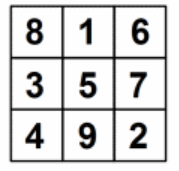
\includegraphics{solution_1}
\centering
\end{figure}

One can see from the figure above that a magic square is a set of spaces filled with integers arranged in a matrix of $n$ by $n$ spaces where $n$ is some natural number. This project solely deals with the special case where $n = 3$ as above. \\

The non-trivial property of magic squares is that each row, column, and diagonal sum to the same number, the so called ``magic sum'' for the specific board. Another property to notice is that the board above only uses the numbers 1 through 9, or 1 through the total number of spaces on the board. While this property is not vital for all magic squares, this is another constraint we have put on this project, otherwise the number of possible boards would be infinite. 

\subsubsection{Properties of 3x3 Magic Squares}

Here we can mention some of the mathematical properties of 3x3 magic squares. We start by stating there are exactly 8 solutions to a 3x3 board, enumerated here:

\begin{figure} [h]
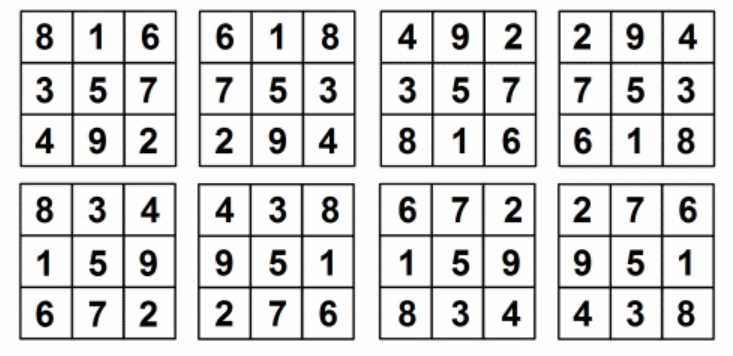
\includegraphics{solutions}
\centering
\end{figure}

These solutions come from the constraint that we can only use the numbers 1 through 9. As such, our magic sum is permanently 15. Further, there are only 8 combinations of numbers which sum to 15, which results in our 8 solutions. \\

\subsubsection{Magic Squares as Puzzles}

Now that we understand the properties that make a magic square a magic square, we can start to see how we can make one of these a puzzle. We do this by simply hiding spaces from the solution to the solver of our puzzle for the solver to fill in, such as what follows:

\begin{figure} [h]
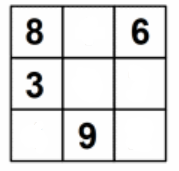
\includegraphics{puzzle_1}
\centering
\end{figure}

An important property to notice is that this board does not hide {\it too} many spaces. While we could hide all of the spaces from the solver and the solver could in theory solve such a puzzle, we do not want to do that for the purposes of our puzzle creation. The puzzles we want to create should have {\it unique solutions}, that is there is exactly one solution to the puzzle we give to the solver. From here on out a puzzle with a unique solution is referred to as a unique puzzle.

\subsubsection{Enumerating Unique Puzzles}

Now we can start looking at the properties these solutions holds as it pertains to creating valid unique puzzles. As one considers the number of possible unique puzzles, the question begins to arise of when exactly does a puzzle cease to be unique? If we hide all of the spaces from the solver the puzzle is clearly not unique, and if we hide none of the space from the solver the puzzle is clearly unique. How many spaces then can we hide from the solver before the puzzle becomes non unique? \\

The answer is definitely a non trivial one, and rests at the heart of how we will eventually generate these puzzles. So we begin by noticing a key property to all of the solutions: the middle space is 5. With this in mind, there are therefore only 8 spaces which we can hide and continue to claim that our puzzle is unique. For our purposes, the middle space is always hidden for our generated puzzles. \\

Now that we have that established, we can begin to notice another important fact: if we leave 3 spaces revealed excluding the middle space, our puzzle will be unique. That is to say all puzzles with the middle space and up to 5 additional spaces hidden are unique. \\

We see then that we now have only 2 spaces revealed excluding the middle space. Here we then define corners and edges: corners are exactly that of the board and edges are all outside space which are not the corners. If we refer to the enumerated solutions above, and specifically the first board enumerated, each pair of opposite corners and opposite edges is shared with another solution. For example if we look at the pair of opposite edges as follows:

\begin{figure} [h]
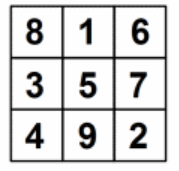
\includegraphics{solution_1}
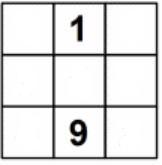
\includegraphics{example_2}
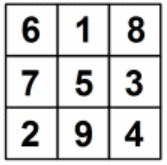
\includegraphics{example_3}
\centering
\end{figure}

These are the only cases where we need to be careful. Excluding the middle space: all puzzles with 1 or 0 spaces revealed are non unique, all puzzles with 3 to 8 spaces revealed are unique, and those puzzles with exactly 2 spaces revealed are unique only if the 2 spaces revealed are not a pair of opposite corners nor edges.

\subsection{SPIN}

Now we describe the tool used to tackle the problem of solving and generating such puzzles. SPIN is an explicit model checking tool which uses a C-like modeling language, PROMELA, to create and analyze the model being described. This section describes the most notable properties of SPIN that affected the project. Documentation for SPIN and its companion language PROMELA can be found here: \url{http://spinroot.com/spin/Man/}.

\subsubsection{Syntax}
As described above,  the syntax for the modeling language is very C-like. This comes with many advantages. The arguably primary advantage of this is that it more easily allows for the modeling on concurrent processes. However, for the purposes of this project, that is not what makes the language so useful. What makes it most useful is that while building the model, one can  use fairly traditional programming techniques without having to simply enumerate what states exist. The model for this project uses this property extensively.

\subsubsection{State Space}
An important behavior to point out with explicit model checking is that the tools explicitly build the entire state space which a model exhibits. This is important to understand for later, as this behavior can lead to serious complications with a model in the form of state space explosion. That is if one does not discriminate when building their model or their model simply exhibits too many potential states, then the model checker may not be able to reason over the entire model as it is intended to do.

\subsubsection{Never Claims}
SPIN reasons over the entire state space for a model, clearly, but how is this useful? One way this is useful is by utilizing assertions. SPIN specifically uses assertions to reason over how a certain set of states should {\it never} occur in a model. This is especially and most clearly useful to describe safety critical systems, wherein certain properties should always or never hold. SPIN will use these assertions which the user can define, called never claims in this case, to provide a counter example and trace of a model if the never claim we provide is ever violated. This property is one of the primary reasons SPIN is so powerful.

\section{Modeling Magic Squares in SPIN}

Now that we have established the various properties of magic squares and the model checker we will be using, we can begin to describe how exactly we modeled 3x3 magic squares in SPIN. We also will begin this discussion by focusing solely on the question of how to generate these puzzles, since once we have the model built to generate them we can use the same model to solve them.

\subsection{Defining the State Space}
As previously mentioned, SPIN explicitly describes and reasons over the entire state space of a model. Given this, it follows that if we are looking to generate puzzles, we should create a model which describes the set of all unique puzzles since any non unique puzzle is of no use to us. \\

If we refer to the previous discussion about magic squares, the most helpful assertion that will help us to define our state space is that, excluding the middle space, those puzzles with 3 to 8 spaces revealed are all unique and those puzzles with exactly 2 spaces revealed are unique only if the 2 spaces revealed are not a pair of opposite corners nor edges. This assertion therefore describes our model's exact intended state space. Here we will also briefly mention that once we have this model built, we can use the special case where all 9 spaces are revealed to solve these puzzles. \\

\subsection{The Model}
We then begin looking at how we describe our intended model in PROMELA. The strategy to creating the desired state space is to start with 2 data sets: firstly is an empty array of 9 integers to describe the board which is currently being reasoned over (indexing is described in Figure 1 below), and secondly the set of 8 solutions which will be used to construct our output board from. The set of solution boards are described using the {\it typedef} data structure. \\

\begin{figure} [h]
\centering
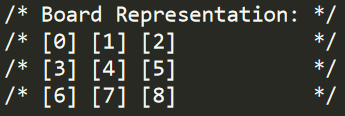
\includegraphics{board_indexing}
\caption{ Board Indexing }
\end{figure}

From here we initialize the model by filling the set of solution boards as they are represented above and runs the process {\it generate()}. This process does exactly as its name describes and generates the intended state space for our model.\\

A few notes before we describe the {\it generate()} process: the model uses a few values to determine which board SPIN will give as a counterexample. These values are the {\it spaces\_filled}, {\it difficulty}, and {\it seed} values. The first two values do essentially the same thing, the {\it difficulty} value simply also discriminates against those boards which have either 2 corners or edges or a corner edge combination. The {\it seed} value is a number from 0 to 7 which determines which solution board the output is choosing its spaces to reveal from.

\subsubsection{The Generate Process}

There are 3 sections to the {\it generate} process: one for iterating the boards which are 2 corners or 2 edges, one for iterating the boards which have a corner edge combination, and one for boards with more than 2 spaces filled. The general way in which we iterate boards can be seen in a portion of the first section of our process:

\begin{figure} [h]
\centering
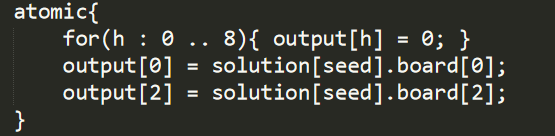
\includegraphics{section_1}
\end{figure}

This section first resets the output board to be all zeroes, then fills the board with the corresponding pair of corners or edges. There are only 8 unique corner or edge pairs as follows: $(0,2), (0,6), (1,3), (1,5), (2,8), (3,7), (5,7), (6,8)$. We only enumerate these combinations since there is no way that was found to relate the indexes described. \\

The second section deals with puzzles with a corner edge combination. The important fact to note for this section is that corners have even indexes and edges have odd indexes. The model uses nested for loops to pick the first and second indices to take from the chosen solution board. \\

The final section uses an array which stores the numbers 0 to 3 and 5 to 8, or the valid indices to choose from the solution board. The model then chooses 3 of these values, removes them from the array, and places those indices from the selected solution board into our output board. After this, the model chooses however many more spaces the user specifies and fills the output board accordingly. \\

Please refer to Appendix section A for the models described above.

\subsection{Valid Never Claims}
Here is when the fun begins. We will then use never claims to generate boards of our choosing. Notable about this is that we can generate whatever board we so desire and eventually solve any board simply by modifying the never claim. There are a few specifications we have to specify for our model to generate these puzzles, however. They are as follows: 

\begin{enumerate}
\item The {\it seed} value
\item The {\it spaces\_filled} value
\item The spaces which you would like you have a value in them
\end{enumerate}

We need to the {\it seed} value to add a bit of randomness, otherwise the solution to our puzzle will be the same every time, if left unspecified. The {\it spaces\_filled} value is how many spaces we want the puzzle to have revealed for our solver. And at this point the model requires us to define which spaces we would like to have filled, though this requirement can be taken away with some minor tweaking to the model. Also of note, as of now the {\it spaces\_filled} value and the number of spaces you specify to look for on the board must match. This is a property that should not hold but can be worked out later. \\

An example of a never claim to describe a board with the top row filled is as follows:

\begin{figure} [h]
\centering
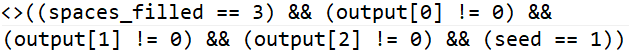
\includegraphics{never_claim}
\end{figure}

Notice the entire LTL statement is enclosed in an {\it eventually} operator. SPIN takes this statement and negates it, thus asserting that what is inside of our {\it eventually} operator {\it always does not} occur, or {\it never} occurs. Thus when we verify our model with this never claim, SPIN will predictably output an error for an assertion violation and a counterexample once it has found a board which matches our description from the LTL statement. \\

Also worth noting is that we use the {\it not equals} operator when we define which spaces should be filled. This is because the board defaults to all 0s, so once a number for that space is selected it is no longer 0. \\

Now if we place this never claim in a .ltl file and run the following commands, we will get an outputted board that will meet our specifications: 

\begin{figure} [h]
\centering
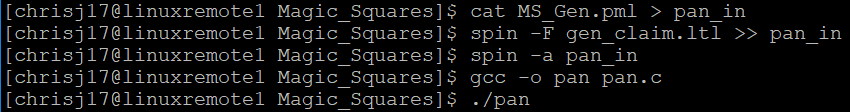
\includegraphics{commands_1}
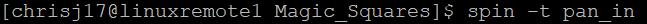
\includegraphics{commands_2}
\end{figure}

The outputted board comes in the following format and corresponds to the respective puzzle:

\begin{figure} [h]
\centering
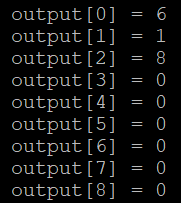
\includegraphics{commands_3}
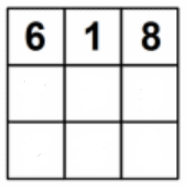
\includegraphics{board_1}
\end{figure}

\newpage

\subsubsection{Solving Puzzles}
Now we expand the model to allow the user to solve any puzzle. We do this by adding a section to the model which copies each solution board into the output board. If we then specify that there are 9 spaces to be filled in our output and that certain spaces are the values which are presented in the puzzle, SPIN will output the solution. \\

The following specification outputs the corresponding board:

\begin{figure} [h]
\centering
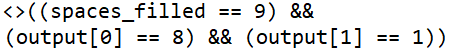
\includegraphics{solved_spec}
\end{figure}

\begin{figure} [h]
\centering
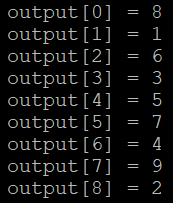
\includegraphics{solution_2}
\end{figure}

\subsection{Model Validation}
Now we turn to the question of validation. How do we ensure the model models the state space we want and nothing more?

\subsubsection{Removing Portions of the Model}
Three ways in which the model was validated was by removing the three sections of the {\it generate()} process as described above and verifying the model with a never claim that should be violated by the section that deals with it. For example, we can use the following specification over a model with the first section of our {\it generate()} process removed to ensure SPIN does not find a violation.

\begin{figure} [h]
\centering
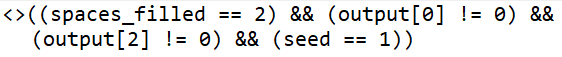
\includegraphics{never_claim_2}
\end{figure}

This property holds true for when we remove each section create its respective LTL claim.

\newpage

\subsubsection{Invalid Never Claims}
We can also run invalid never claims and ensure SPIN does not find a violation. One way this can be done is by taking the following specification and running SPIN over our model with it as our never claim: 

\begin{figure} [h]
\centering
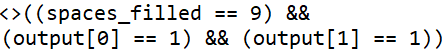
\includegraphics{validation_1}
\end{figure}

\section{Conclusion and Future Work}
We conclude this final report by asserting that the project has been a success. There is clearly more work to do with the model, however. One can clearly see that the model has not yet been validated nearly enough to claim that it reasons strictly over the state space we claim it does. Therefore more validation is needed to ensure the model works only as intended. \\

To that end the model also needs more refinement. Much of the model was built in a fairly short amount of time, as the project pivoted very quickly at the tail end of its timeline. There is likely a more clever way to build the model the way that it was done. Notably dealing with ignoring the fourth index of every board since it was always 5. This caused a lot of what is likely unnecessary complexity to the model. \\

Overall the model does what it set out to do, to solve and generate 3x3 magic square puzzles. While it may be a little sloppy and can certainly be refined, it gets the job done in a fairly user friendly way.

\newpage

\appendix
\section{GitHub Repository}
This report and all source code including models and specifications can be found on a public GitHub repository at:\\ \url{https://github.com/chrisj3/aere407-final-project-magic-SPIN-solver}

\section{Magic Square Math}
Much of the inspiration for taking this model in the direction it is going now can be found at this website: \url{https://www.grogono.com/magic/index.php}, which includes a lot of the very interesting mathematics behind magic squares.

\end{document}